%iffalse
\let\negmedspace\undefined
\let\negthickspace\undefined
\documentclass[journal,12pt,onecolumn]{IEEEtran}
\usepackage{cite}
\usepackage{amsmath,amssymb,amsfonts,amsthm}
\usepackage{algorithmic}
\usepackage{graphicx}
\usepackage{textcomp}
\usepackage{xcolor}
\usepackage{txfonts}
\usepackage{listings}
\usepackage{enumitem}
\usepackage{mathtools}
\usepackage{gensymb}
\usepackage{comment}
\usepackage[breaklinks=true]{hyperref}
\usepackage{tkz-euclide} 
\usepackage{listings}
\usepackage{gvv}                                        
%\def\inputGnumericTable{}                                 
\usepackage[latin1]{inputenc}                                
\usepackage{color}                                            
\usepackage{array}                                            
\usepackage{longtable}                                       
\usepackage{calc}                                             
\usepackage{multirow}                                         
\usepackage{hhline}                                           
\usepackage{ifthen}                                           
\usepackage{lscape}
\usepackage{tabularx}
\usepackage{array}
\usepackage{float}


\newtheorem{theorem}{Theorem}[section]
\newtheorem{problem}{Problem}
\newtheorem{proposition}{Proposition}[section]
\newtheorem{lemma}{Lemma}[section]
\newtheorem{corollary}[theorem]{Corollary}
\newtheorem{example}{Example}[section]
\newtheorem{definition}[problem]{Definition}
\newcommand{\BEQA}{\begin{eqnarray}}
\newcommand{\EEQA}{\end{eqnarray}}
\newcommand{\define}{\stackrel{\triangle}{=}}
\theoremstyle{remark}
\newtheorem{rem}{Remark}

% Marks the beginning of the document
\begin{document}
\bibliographystyle{IEEEtran}
\vspace{3cm}

\title{1-1.6.16}
\author{AI24BTECH11011 - Himani Gourishetty}
\maketitle
\bigskip

\renewcommand{\thefigure}{\theenumi}
\renewcommand{\thetable}{\theenumi}
\begin{enumerate}
\item Find the values of k if the points $\vec{A}\brak{k+1,2k}$ , $\vec{B}\brak{3k,2k+3}$ , $\vec{C}\brak{5k-1,5k}$ are collinear.\\
\textbf{Solution} Given,\\
\begin{table}[h!]    
\centering
\begin{tabular}[12pt]{ |c|c|c|}
\hline
\textbf{Variable} & \textbf{Description} & \textbf{formula}\\ 
\hline
$\vec{A}\brak{x1,y1}$ & $\brak{k+1,2k}$  & - \\
\hline 
$\vec{B}\brak{x2,y2}$ & $\brak{3k,2k+3}$ & - \\
\hline
$\vec{C}\brak{x3,y3}$ & $\brak{5k-1,5k}$ & - \\
\hline 
Area & Area formed by the 3 points & $x1\brak{y2-y3}+x2\brak{y3-y1}+x3\brak{y1-y2}\\
\hline
\end{tabular}

\label{q3}
\end{table}\\
For Points $\vec{A},\vec{B},\vec{C}$ to be collinear if
\begin{align}
    rank \myvec{\vec{B}-\vec{A} & \vec{C}-\vec{A}} & = 1\\
    \vec{B}-\vec{A} = \myvec{3k \\ 2k+3} - \myvec{k+1 \\ 2k}\\
    = \myvec{2k-1 \\ 3}\\
    \vec{C}-\vec{A} = \myvec{5k-1\\5k}-\myvec{k+1\\2k}\\
  = \myvec{4k-2\\3k}\\
  \myvec{\vec{B}-\vec{A} & \vec{C}-\vec{A}} =\myvec{2k-1 & 4k-2 \\ 3 & 3k}\\
  \end{align}
  Now, rank of this matrix should be 1.
  \begin{align}
  \myvec{2k-1 & 4k-2 \\ 3 & 3k} &\xrightarrow[]{R_2\rightarrow R_2 - R_1} \myvec{2k-1 & 4k-2 \\ 4-2k & -k+2}\\
  rank\myvec{2k-1 & 2\brak{2k-1} \\ -2\brak{-k+2} & -k+2}=1\\
  \end{align}
  For the rank to be one, either of below should be true,
  \begin{align}
  2k-1=0 \\
  -k+2=0
\end{align}
then,
\begin{align}
k=2;
k=0.5   
\end{align}
\begin{figure}[ht]
   \centering
   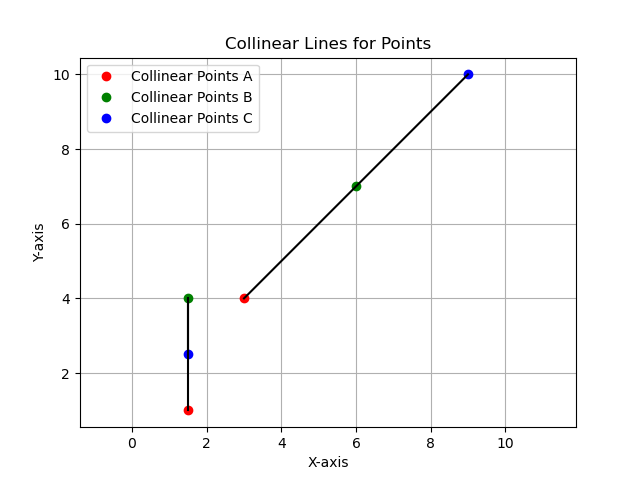
\includegraphics[width=0.7\linewidth]{figs/Figure_1.png}
   \label{q31}
\end{figure}


\end{document}
